%  LaTeX support: latex@mdpi.com
%  For support, please attach all files needed for compiling as well as the log file, and specify your operating system, LaTeX version, and LaTeX editor.

%=================================================================
% pandoc conditionals added to preserve backwards compatibility with previous versions of rticles

\documentclass[Water,article,submit,oneauthor]{Definitions/mdpi}


%% Some pieces required from the pandoc template
\setlist[itemize]{leftmargin=*,labelsep=5.8mm}
\setlist[enumerate]{leftmargin=*,labelsep=4.9mm}


%--------------------
% Class Options:
%--------------------

%---------
% article
%---------
% The default type of manuscript is "article", but can be replaced by:
% abstract, addendum, article, book, bookreview, briefreport, casereport, comment, commentary, communication, conferenceproceedings, correction, conferencereport, entry, expressionofconcern, extendedabstract, datadescriptor, editorial, essay, erratum, hypothesis, interestingimage, obituary, opinion, projectreport, reply, retraction, review, perspective, protocol, shortnote, studyprotocol, systematicreview, supfile, technicalnote, viewpoint, guidelines, registeredreport, tutorial
% supfile = supplementary materials

%----------
% submit
%----------
% The class option "submit" will be changed to "accept" by the Editorial Office when the paper is accepted. This will only make changes to the frontpage (e.g., the logo of the journal will get visible), the headings, and the copyright information. Also, line numbering will be removed. Journal info and pagination for accepted papers will also be assigned by the Editorial Office.

%------------------
% moreauthors
%------------------
% If there is only one author the class option oneauthor should be used. Otherwise use the class option moreauthors.

%---------
% pdftex
%---------
% The option pdftex is for use with pdfLaTeX. Remove "pdftex" for (1) compiling with LaTeX & dvi2pdf (if eps figures are used) or for (2) compiling with XeLaTeX.

%=================================================================
% MDPI internal commands - do not modify
\firstpage{1}
\makeatletter
\setcounter{page}{\@firstpage}
\makeatother
\pubvolume{1}
\issuenum{1}
\articlenumber{0}
\pubyear{2023}
\copyrightyear{2023}
%\externaleditor{Academic Editor: Firstname Lastname}
\datereceived{ }
\daterevised{ } % Comment out if no revised date
\dateaccepted{ }
\datepublished{ }
%\datecorrected{} % For corrected papers: "Corrected: XXX" date in the original paper.
%\dateretracted{} % For corrected papers: "Retracted: XXX" date in the original paper.
\hreflink{https://doi.org/} % If needed use \linebreak
%\doinum{}
%\pdfoutput=1 % Uncommented for upload to arXiv.org

%=================================================================
% Add packages and commands here. The following packages are loaded in our class file: fontenc, inputenc, calc, indentfirst, fancyhdr, graphicx, epstopdf, lastpage, ifthen, float, amsmath, amssymb, lineno, setspace, enumitem, mathpazo, booktabs, titlesec, etoolbox, tabto, xcolor, colortbl, soul, multirow, microtype, tikz, totcount, changepage, attrib, upgreek, array, tabularx, pbox, ragged2e, tocloft, marginnote, marginfix, enotez, amsthm, natbib, hyperref, cleveref, scrextend, url, geometry, newfloat, caption, draftwatermark, seqsplit
% cleveref: load \crefname definitions after \begin{document}

%=================================================================
% Please use the following mathematics environments: Theorem, Lemma, Corollary, Proposition, Characterization, Property, Problem, Example, ExamplesandDefinitions, Hypothesis, Remark, Definition, Notation, Assumption
%% For proofs, please use the proof environment (the amsthm package is loaded by the MDPI class).

%=================================================================
% Full title of the paper (Capitalized)
\Title{HYDROLOGICAL IMPACTS OF PATCH CUTTING}

% MDPI internal command: Title for citation in the left column
\TitleCitation{HYDROLOGICAL IMPACTS OF PATCH CUTTING}

% Author Orchid ID: enter ID or remove command
%\newcommand{\orcidauthorA}{0000-0000-0000-000X} % Add \orcidA{} behind the author's name
%\newcommand{\orcidauthorB}{0000-0000-0000-000X} % Add \orcidB{} behind the author's name


% Authors, for the paper (add full first names)
\Author{Ming
Qiu$^{1,\ddagger,*}$\href{https://orcid.org/0000-0002-3755-7465}
{\orcidicon}}


%\longauthorlist{yes}


% MDPI internal command: Authors, for metadata in PDF
\AuthorNames{Ming Qiu}

% MDPI internal command: Authors, for citation in the left column

% Affiliations / Addresses (Add [1] after \address if there is only one affiliation.)
\address{%
$^{1}$ \quad University of British Columbia Okanagan - Department of
Earth, Environmental and Geographic Sciences 1177 Research Road,
Kelowna, BC, Canada, V1V
1V7; \href{mailto:ming.qiu@ubc.ca}{\nolinkurl{ming.qiu@ubc.ca}}\\
}

% Contact information of the corresponding author
\corres{Correspondence: \href{mailto:ming.qiu@ubc.ca}{\nolinkurl{ming.qiu@ubc.ca}};
Tel.: +XX-000-00-0000.}

% Current address and/or shared authorship








% The commands \thirdnote{} till \eighthnote{} are available for further notes

% Simple summary
\simplesumm{A Simple summary goes here.}

%\conference{} % An extended version of a conference paper

% Abstract (Do not insert blank lines, i.e. \\)
\abstract{This project aims to monitor forest stand-level environmental
variables related to hydrological processes along forest
interior-edge-cutblock transects. The research questions to be addressed
include: (1) what environmental variables exhibit an observable gradient
from forest edges to forest interiors? (2) How can hydrological
processes such as flow path, evapotranspiration be affected along the
transects? Monitoring and sampling will be carried out along forest
edges adjacent to fresh cutblocks (i.e., harvest year ≥ 2020). The
dataset for this research component will encompass various environmental
variables, soil moisture, and soil water isotope signatures.
Environmental variables and soil moisture will be continuously
monitored, with measurements taken every hour using
microcontroller-based sensors (specifically, Arduino Pro Mini).
Considering that edge effects can extend up to two to three times the
tree height, microcontrollers will be strategically placed: at the edge,
15 m and 30 m from the edge in both opening and interior positions. Soil
sampling will be consistent across these locations, targeting depths of
15 cm and 30 cm. Anticipated results include (1) remarkable differences
in residence time distributions of soil water between forests and
disturbed areas, indicative of distinct prevailing flow paths; (2)
notable gradients in soil moisture, temperature, relative humidity, and
solar radiation along forest interior-edge-opening transects, which can
account for the affected evaporation processes.}


% Keywords
\keyword{mock; Rmarkdown; Ecohydrology}

% The fields PACS, MSC, and JEL may be left empty or commented out if not applicable
%\PACS{J0101}
%\MSC{}
%\JEL{}

%%%%%%%%%%%%%%%%%%%%%%%%%%%%%%%%%%%%%%%%%%
% Only for the journal Diversity
%\LSID{\url{http://}}

%%%%%%%%%%%%%%%%%%%%%%%%%%%%%%%%%%%%%%%%%%
% Only for the journal Applied Sciences

%%%%%%%%%%%%%%%%%%%%%%%%%%%%%%%%%%%%%%%%%%

%%%%%%%%%%%%%%%%%%%%%%%%%%%%%%%%%%%%%%%%%%
% Only for the journal Data



%%%%%%%%%%%%%%%%%%%%%%%%%%%%%%%%%%%%%%%%%%
% Only for the journal Toxins


%%%%%%%%%%%%%%%%%%%%%%%%%%%%%%%%%%%%%%%%%%
% Only for the journal Encyclopedia


%%%%%%%%%%%%%%%%%%%%%%%%%%%%%%%%%%%%%%%%%%
% Only for the journal Advances in Respiratory Medicine
%\addhighlights{yes}
%\renewcommand{\addhighlights}{%

%\noindent This is an obligatory section in “Advances in Respiratory Medicine”, whose goal is to increase the discoverability and readability of the article via search engines and other scholars. Highlights should not be a copy of the abstract, but a simple text allowing the reader to quickly and simplified find out what the article is about and what can be cited from it. Each of these parts should be devoted up to 2~bullet points.\vspace{3pt}\\
%\textbf{What are the main findings?}
% \begin{itemize}[labelsep=2.5mm,topsep=-3pt]
% \item First bullet.
% \item Second bullet.
% \end{itemize}\vspace{3pt}
%\textbf{What is the implication of the main finding?}
% \begin{itemize}[labelsep=2.5mm,topsep=-3pt]
% \item First bullet.
% \item Second bullet.
% \end{itemize}
%}


%%%%%%%%%%%%%%%%%%%%%%%%%%%%%%%%%%%%%%%%%%


% tightlist command for lists without linebreak
\providecommand{\tightlist}{%
  \setlength{\itemsep}{0pt}\setlength{\parskip}{0pt}}



\usepackage{longtable}

\begin{document}



%%%%%%%%%%%%%%%%%%%%%%%%%%%%%%%%%%%%%%%%%%

\hypertarget{introduction}{%
\section{Introduction}\label{introduction}}

Numerous studies across the world have unveiled the intricate
relationship between forests and water
\citep{bertrand-krajewski_distribution_1998, leutnant_stormwater_2016}.This
profound connection arises from the crucial role that forests play in
the water cycle, affecting not only water supply in both social and
natural systems but also aquatic habitat and biodiversity conservation.

In British Columbia (BC), where forests cover nearly 64\% of the land,
watershed management practices involve dealing with a range of forest
disturbances from anthropogenic disturbances (e.g., timber harvesting,
agriculture) to natural disturbances (e.g., insect infestation,
wildfire). Over the past decades, there have been a fair number of
studies addressing the forest-water relationship, which confirmed forest
cover changes are significantly associated with alterations in
streamflow, posing a noticeable threat to water supply.

Literature suggests that\ldots{} (Figure \ref{fig:fig1})

\begin{figure}
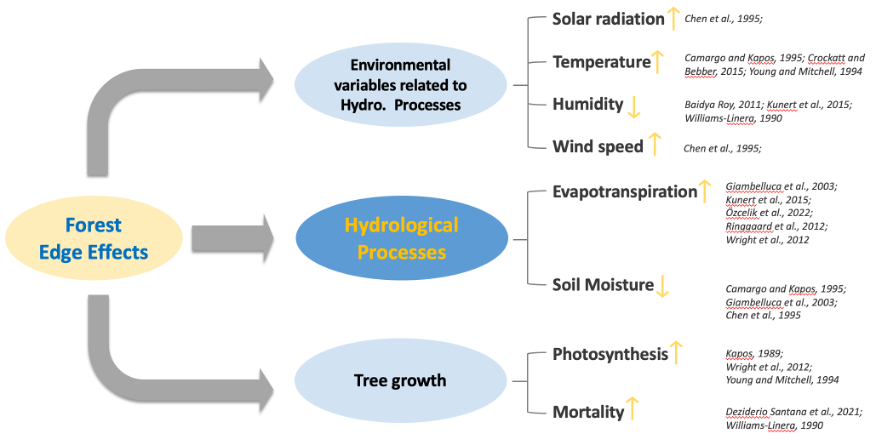
\includegraphics[width=0.7\linewidth]{../04_figs/literature_summary} \caption{A figure added from a folder.\label{fig:fig1}}\label{fig:fig1}
\end{figure}

\hypertarget{materials-and-methods}{%
\section{Materials and Methods}\label{materials-and-methods}}

\hypertarget{study-area}{%
\subsection{Study area}\label{study-area}}

Our study area is the Duteau community watershed, located approximately
20 km southeast of the City of Vernon (Figure S1). It has a total
drainage area of 213 km2, ranging in elevation from 520 m at its
confluence with Bessette Creek to over 1,800 m in the Grizzly Hills. It
is a snow-dominated system with peak flows occurring from late-April to
mid-June. Since the 1890's, the watershed has been developed for
irrigation and water supplies, providing 60 per cent of Vernon's
drinking water and serving a population in the Greater Vernon area of
more than 50,000 \#\# Data processing and analysis Processes include: 1.
First step 2. Second step 3. Third step

\hypertarget{data-analysis}{%
\subsection{Data analysis}\label{data-analysis}}

\begin{equation}
E = MC^2
\end{equation}

\hypertarget{results}{%
\section{Results}\label{results}}

Results suggested (see \ref{fig:fig2} and \ref{tab:tab1}):

\begin{itemize}
\tightlist
\item
  First bullet
\item
  Second bullet
\item
  Third bullet
\end{itemize}

\begin{figure}
\centering
\includegraphics{LDP_manuscript_v1_files/figure-latex/fig2-1.pdf}
\caption{A figure added with a code chunk.\label{fig:fig2}}
\end{figure}

\begin{table}[H]

\caption{\label{tab:tab1}Table created based on mtcars.}
\begin{tabular}[t]{lccc}
\toprule
  & mpg & cyl & disp\\
\midrule
Mazda RX4 & 21.0 & 6 & 160\\
Mazda RX4 Wag & 21.0 & 6 & 160\\
Datsun 710 & 22.8 & 4 & 108\\
Hornet 4 Drive & 21.4 & 6 & 258\\
Hornet Sportabout & 18.7 & 8 & 360\\
\bottomrule
\end{tabular}
\end{table}

\hypertarget{discussion}{%
\section{Discussion}\label{discussion}}

The results are consistent with the previous findings \ldots{}

\hypertarget{conclusion}{%
\section{Conclusion}\label{conclusion}}

We conclude that\ldots{}

%%%%%%%%%%%%%%%%%%%%%%%%%%%%%%%%%%%%%%%%%%

\vspace{6pt}

%%%%%%%%%%%%%%%%%%%%%%%%%%%%%%%%%%%%%%%%%%
%% optional

% Only for the journal Methods and Protocols:
% If you wish to submit a video article, please do so with any other supplementary material.
% \supplementary{The following supporting information can be downloaded at: \linksupplementary{s1}, Figure S1: title; Table S1: title; Video S1: title. A supporting video article is available at doi: link.}

%%%%%%%%%%%%%%%%%%%%%%%%%%%%%%%%%%%%%%%%%%

\funding{This research was funded by NSERC xxxx.}


\informedconsent{Informed consent was obtained from all subjects
involved in the study.}

\dataavailability{Data available in OSF project
\url{https://osf.io/khs4q/?view_only=a7e4c843de094544a75872da5680edd3}}

\acknowledgments{Thank all very much}

\conflictsofinterest{The authors declare no conflict of interest.}

%%%%%%%%%%%%%%%%%%%%%%%%%%%%%%%%%%%%%%%%%%
%% Optional

%% Only for journal Encyclopedia

\abbreviations{Abbreviations}{
The following abbreviations are used in this manuscript:\\

\noindent
\begin{tabular}{@{}ll}
MDPI & Multidisciplinary Digital Publishing Institute \\
LDP & Living Data Project \\
\end{tabular}}

%%%%%%%%%%%%%%%%%%%%%%%%%%%%%%%%%%%%%%%%%%
%% Optional
\input{"appendix.tex"}
%%%%%%%%%%%%%%%%%%%%%%%%%%%%%%%%%%%%%%%%%%
\begin{adjustwidth}{-\extralength}{0cm}

%\printendnotes[custom] % Un-comment to print a list of endnotes


\reftitle{References}
\bibliography{mybibfile.bib}

% If authors have biography, please use the format below
%\section*{Short Biography of Authors}
%\bio
%{\raisebox{-0.35cm}{\includegraphics[width=3.5cm,height=5.3cm,clip,keepaspectratio]{Definitions/author1.pdf}}}
%{\textbf{Firstname Lastname} Biography of first author}
%
%\bio
%{\raisebox{-0.35cm}{\includegraphics[width=3.5cm,height=5.3cm,clip,keepaspectratio]{Definitions/author2.jpg}}}
%{\textbf{Firstname Lastname} Biography of second author}

%%%%%%%%%%%%%%%%%%%%%%%%%%%%%%%%%%%%%%%%%%
%% for journal Sci
%\reviewreports{\\
%Reviewer 1 comments and authors’ response\\
%Reviewer 2 comments and authors’ response\\
%Reviewer 3 comments and authors’ response
%}
%%%%%%%%%%%%%%%%%%%%%%%%%%%%%%%%%%%%%%%%%%
\PublishersNote{}
\end{adjustwidth}


\end{document}
